\section{Introduction}


\subsection{Articles}
\begin{frame}{Articles}
    \leftmargini=0pt
    \begin{itemize}
        \item \textbf{(2008) Fab-map: Probabilistic localization and mapping in the space of appearance}~\cite{fabmap2008b} ;
        \item (2009) Accelerating fab-map with concentration inequalities~\cite{accelerating} ;
        \item (2010) Fab-map 3d : Topological mapping with spatial and visual appearance~\cite{fabmap3d} ;
        \item \textbf{(2011) Appearance-only slam at large scale with fab-map~2.0}~\cite{fabmap2011} ;
        \item \textbf{(2012) Openfabmap : An open source toolbox for appearance-based loop closure detection}~\cite{openfabmap}.
    \end{itemize}
    \note[item]{Context ... Long sequences of FAB-MAP related articles...}
    \note[item]{Article getting OLD -- 2008, but...}
    \note[item]{For 1.0 and 2.0 Conference version first, then version journal}
    \note[item]{Non exaustive list... I might forget some}
\end{frame}

\subsection{FAB-MAP}
\begin{frame}{FAB-MAP}
    \begin{quotation}
        This paper describes a \textbf{probabilistic approach} to the problem of \textbf{recognizing places} based on their \textbf{appearance}. The system we present is not limited to localization, but \textbf{can determine that a new observation comes from a previously unseen place}, and so augment its map. Effectively this is a \textbf{SLAM} system in the space of appearance.~\cite{fabmap2008b}
    \end{quotation}
    \note[item]{Read it first}
    \note[item]{Place recognition}
    \note[item]{Appearance, using visual features from camera as oposed to geometrical features}
    \note[item]{New observation != Localization (simple nearest neighbour)}
    \note[item]{SLAM ? I'll let you decide (counter-intuitive or incomplete)}
\end{frame}

\subsection{Basic Concepts}
\begin{frame}{Basic concepts}
    \begin{itemize}
        \item Map: metric vs topological
        \item \textbf{Simultaneous Localization And Mapping (SLAM)}
        \item Loop closure
        \item Perceptual aliasing
        \item Kidnapped robot
        \item Multi-session mapping
    \end{itemize}
    \note[item]{I will introduce some basics concepts... Do not read all points}
    \note[item]{I give more information than I really need here, but I think it is good for general robotics knowledge}
    \note[item]{Also, introduction+fabmap 1.0 apply to all 3 articles (summary in all)}
\end{frame}

\begin{frame}{Map: Metric vs Topological}
    \begin{figure}
        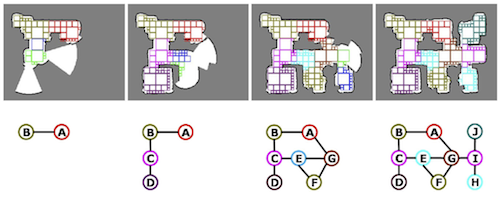
\includegraphics[width=1.0\textwidth]{./media/metric_vs_topo.png}
        \caption{\tiny Source: http://www.autonomousrobotsblog.com/}
    \end{figure}
    \note[item]{Metric (distance between all members)}
    \note[item]{Topological (set of points, along with a set of neighbourhoods for each point)}
    \note[item]{Topological is more abstract... Or if you prefer metric is a specialization of topo}
    \note[item]{There is mathematical definition available if you a fan of it...}
\end{frame}

\begin{frame}{Simultaneous Localization And Mapping (SLAM)}
    \begin{center}
        \href{https://www.youtube.com/watch?v=y7OnimZRj2w}{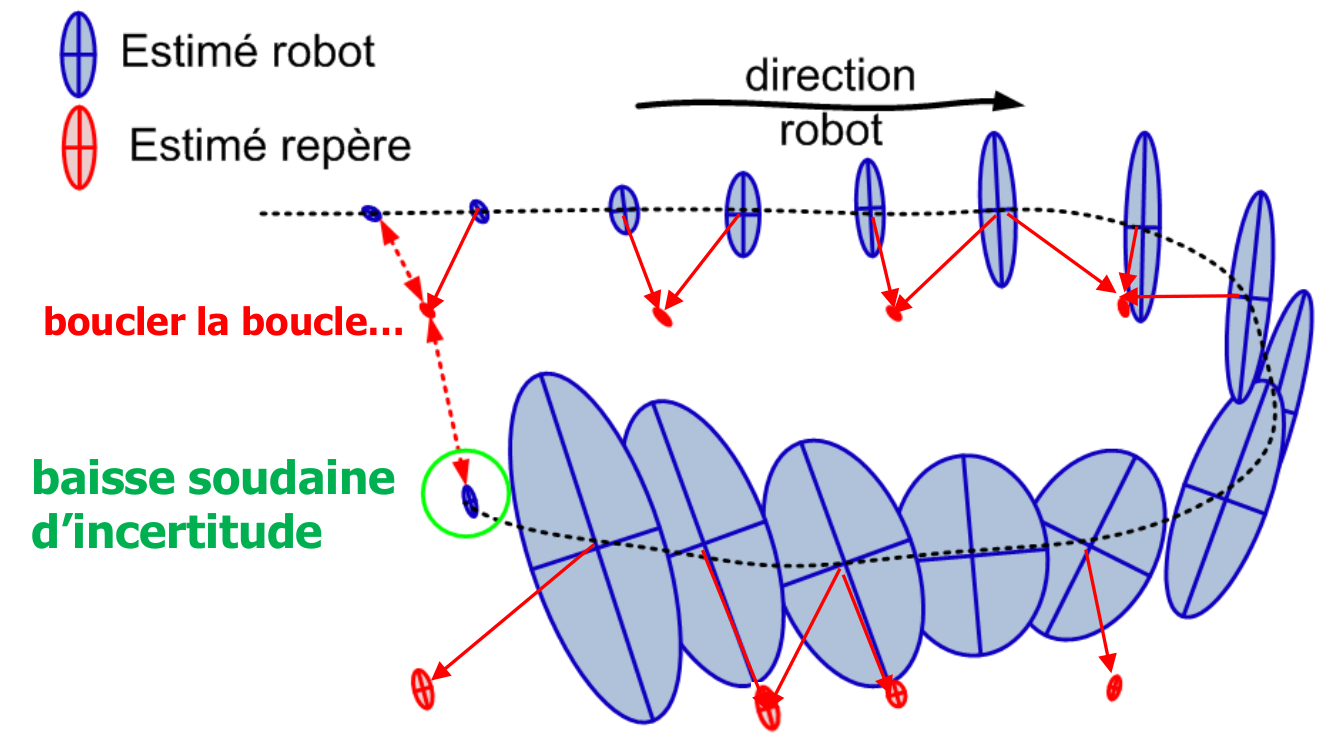
\includegraphics[width=1.0\textwidth]{./media/loop_closure.png}}
        {\tiny Source: GLO-4001/GLO-7021 Introduction à la robotique mobile}
    \end{center}
    \note[item]{Overview: position and features (aka landmark) along with uncertainty/covariance}
    \note[item]{Loop closure... You don't want false positive here ! aka 100\% precision}
\end{frame}

\begin{frame}{Perceptual Aliasing, Kidnapped Robot}
    \begin{columns}
        \begin{column}{0.5\textwidth}
            \begin{center}
                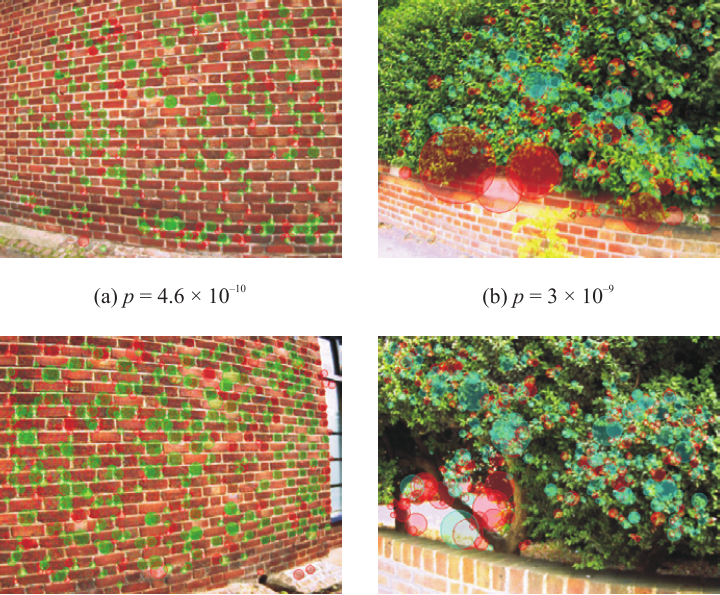
\includegraphics[width=1\textwidth]{./media/perceptual_aliasing2.png}\newline
                {\tiny Source: Fab-map: Probabilistic localization and mapping in the space of appearance~\cite{fabmap2008b}}
            \end{center}
        \end{column}
        \begin{column}{0.5\textwidth}
            \begin{center}
                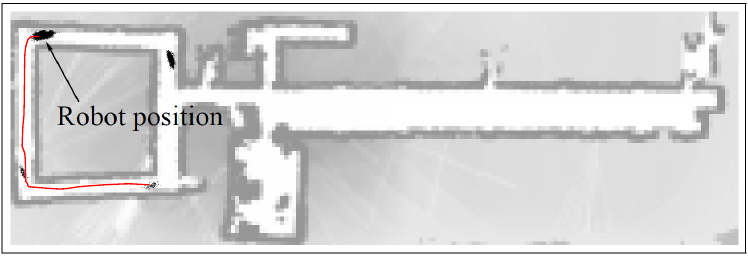
\includegraphics[width=\textwidth]{./media/map1.png}\newline
                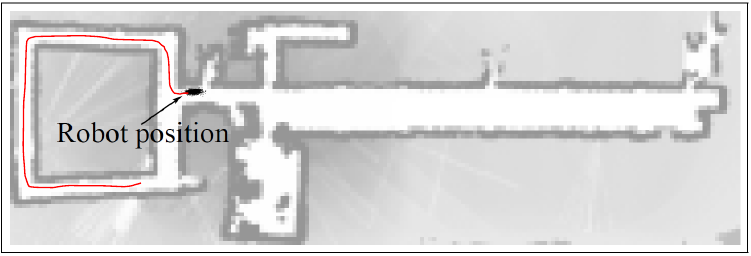
\includegraphics[width=\textwidth]{./media/map2.png}\newline
                {\tiny Source: GLO-4001/GLO-7021 Introduction à la robotique mobile}
            \end{center}
        \end{column}
    \end{columns}
    \note[item]{Perceptual aliasing is simply errors caused by similar appearance}
    \note[item]{Kidnapped Robot ? The robot is teleported somewhere else}
    \note[item]{Why is that a problem ?}
\end{frame}

\begin{frame}{Multi-Session Mapping}
    \begin{center}
        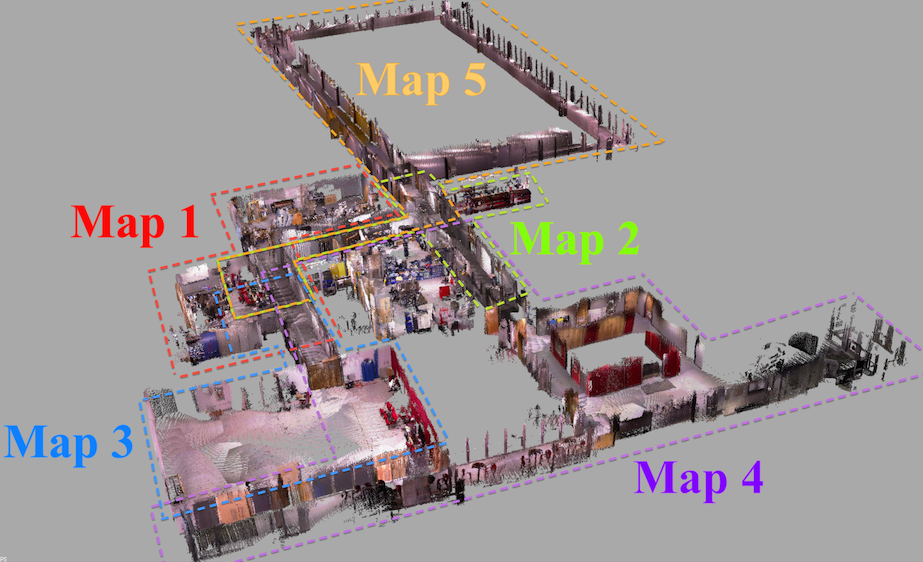
\includegraphics[width=0.85\textwidth]{./media/multi-session.png}\newline
        {\tiny Source: http://introlab.github.io/rtabmap/}
        \note[item]{Multi-session mapping... Combining the results of multiple simultaneous localisation and mapping}
        \note[item]{Therefore you must be able to do place recognition to match overlapping regions}
    \end{center}
\end{frame}

\begin{frame}{Relation with FAB-MAP}
    So...\newline\\
    FAB-MAP does \textbf{place recognition} and \textbf{new place detection} and can therefore be considered as a \textbf{topological SLAM}.\newline\\
    It is \textbf{complementary to metric SLAM}, for which loop closure, kidnapped robot and multi-session mapping problems are challenging.
    \note[item]{Could be seen as a graph where node == place and link means adjacent}
    \note[item]{It is difficult because your current position is often based on the last position}
\end{frame}

